\documentclass[12pt]{article}
\usepackage{amsmath}
\usepackage{amsthm}
\usepackage{amsfonts}
\usepackage{amssymb}
\usepackage{latexsym}
\usepackage{tikz} 
\usepackage{esint} 
%\usepackage{epsfig}
%\usepackage{graphicx}
%\usepackage[dvips]{graphicx}
\usepackage{tikz}
\usepackage{tikz-cd}




\usepackage[matrix,tips,graph,curve]{xy}

\newcommand{\mnote}[1]{${}^*$\marginpar{\footnotesize ${}^*$#1}}
\linespread{1.065}

\makeatletter

\setlength\@tempdima  {5.5in}
\addtolength\@tempdima {-\textwidth}
%\addtolength\hoffset{-0.5\@tempdima}
\addtolength\hoffset{-0.6\@tempdima}
\setlength{\textwidth}{5.5in}
\setlength{\textheight}{8.75in}
%\addtolength\voffset{-0.625in}
\addtolength\voffset{-1.2in}

\makeatother

\makeatletter 
\@addtoreset{equation}{section}
\makeatother


\renewcommand{\theequation}{\thesection.\arabic{equation}}

\theoremstyle{plain}
\newtheorem{theorem}[equation]{Theorem}
\newtheorem{corollary}[equation]{Corollary}
\newtheorem{lemma}[equation]{Lemma}
\newtheorem{proposition}[equation]{Proposition}
\newtheorem{conjecture}[equation]{Conjecture}
\newtheorem{fact}[equation]{Fact}
\newtheorem{facts}[equation]{Facts}
\newtheorem*{theoremA}{Theorem A}
\newtheorem*{theoremB}{Theorem B}
\newtheorem*{theoremC}{Theorem C}
\newtheorem*{theoremD}{Theorem D}
\newtheorem*{theoremE}{Theorem E}
\newtheorem*{theoremF}{Theorem F}
\newtheorem*{theoremG}{Theorem G}
\newtheorem*{theoremH}{Theorem H}

\theoremstyle{definition}
\newtheorem{definition}[equation]{Definition}
\newtheorem{definitions}[equation]{Definitions}
%\theoremstyle{remark}

\newtheorem{remark}[equation]{Remark}
\newtheorem{remarks}[equation]{Remarks}
\newtheorem{exercise}[equation]{Exercise}
\newtheorem{example}[equation]{Example}
\newtheorem{examples}[equation]{Examples}
\newtheorem{notation}[equation]{Notation}
\newtheorem{question}[equation]{Question}
\newtheorem{assumption}[equation]{Assumption}
\newtheorem*{claim}{Claim}
\newtheorem{answer}[equation]{Answer}
%%%%%% letters %%%%

\newcommand{\IA}{\mathbb{A}}
\newcommand{\IB}{\mathbb{B}}
\newcommand{\IC}{\mathbb{C}}
\newcommand{\ID}{\mathbb{D}}
\newcommand{\IE}{\mathbb{E}}
\newcommand{\IF}{\mathbb{F}}
\newcommand{\IG}{\mathbb{G}}
\newcommand{\IH}{\mathbb{H}}
\newcommand{\II}{\mathbb{I}}
\newcommand{\IK}{\mathbb{K}}
\newcommand{\IL}{\mathbb{L}}
\newcommand{\IM}{\mathbb{M}}
\newcommand{\IN}{\mathbb{N}}
\newcommand{\IO}{\mathbb{O}}
\newcommand{\IP}{\mathbb{P}}
\newcommand{\IQ}{\mathbb{Q}}
\newcommand{\IR}{\mathbb{R}}
\newcommand{\IS}{\mathbb{S}}
\newcommand{\IT}{\mathbb{T}}
\newcommand{\IU}{\mathbb{U}}
\newcommand{\IV}{\mathbb{V}}
\newcommand{\IW}{\mathbb{W}}
\newcommand{\IX}{\mathbb{X}}
\newcommand{\IY}{\mathbb{Y}}
\newcommand{\IZ}{\mathbb{Z}}

%%%%%%% macros %%%%%

%% my definitions %%%

\newcommand{\End}{\mathrm{End}}
\newcommand{\tr}{\mathrm{tr}}
%\newcommand{\ind}{\mathrm{ind}}

\renewcommand{\index}{\mathrm{index \,}}
\newcommand{\Hom}{\mathrm{Hom}}
\newcommand{\Aut}{\mathrm{Aut}}
\newcommand{\Trace}{\mathrm{Trace}\,}
\newcommand{\Res}{\mathrm{Res}\,}
%\newcommand{\rank}{\mathrm{rank}}
%\renewcommand{\dim}{\mathrm{dim}}

\renewcommand{\deg}{\mathrm{deg}}
\newcommand{\spin}{\rm Spin}
\newcommand{\supp}{\mathrm{supp \,}}
\newcommand{\Spin}{\rm Spin}
\newcommand{\erfc}{\rm erfc\,}
\newcommand{\sgn}{\rm sgn\,}
\newcommand{\Spec}{\rm Spec\,}
\newcommand{\diag}{\rm diag\,}
\newcommand{\Fix}{\mathrm{Fix}}
\newcommand{\Ker}{\mathrm{Ker \,}}
\newcommand{\Coker}{\mathrm{Coker \,}}
\newcommand{\Sym}{\mathrm{Sym \,}}
\newcommand{\Hess}{\mathrm{Hess \,}}
\newcommand{\grad}{\mathrm{grad \,}}
\newcommand{\Center}{\mathrm{Center}}
\newcommand{\Lie}{\mathrm{Lie}}
\newcommand{\coker}{\mathrm{coker}}

\newcommand{\ch}{\rm ch} % Chern Character

\newcommand{\rank}{\rm rank} 
%\renewcommand{\c}{\rm c}  % Chern class

\newcommand\QED{\hfill $\Box$} %{\bf QED}} 

\newcommand\Pf{\nonintend{\em Proof. }}


\newcommand\reals{{\mathbb R}} 
\newcommand\complexes{{\mathbb C}}
\renewcommand\i{\sqrt{-1}}
\renewcommand\Re{\mathrm Re}
\renewcommand\Im{\mathrm Im}
\newcommand\integers{{\mathbb Z}}
\newcommand\quaternions{{\mathbb H}}


\newcommand\iso{\,{\cong}\,} 
\newcommand\tensor{{\otimes}}
\newcommand\Tensor{{\bigotimes}} 
\newcommand\union{\bigcup} 
\newcommand\onehalf{\frac{1}{2}}
%\newcommand\Sym[1]{{Sym^{#1}(\complexes^2)}}

\newcommand\lie[1]{{\mathfrak #1}} 
\newcommand\smooth{\mathcal{C}^{\infty}}
\newcommand\trivial{{\mathbb I}}
\newcommand\widebar{\overline}

%%%%%Delimiters%%%%

\newcommand{\<}{\langle}
\renewcommand{\>}{\rangle}

%\renewcommand{\(}{\left(}
%\renewcommand{\)}{\right)}


%%%% Different kind of derivatives %%%%%

\newcommand{\delbar}{\bar{\partial}}
\newcommand{\pdu}{\frac{\partial}{\partial u}}
%\newcommand{\pd}[1][2]{\frac{\partial #1}{\partial #2}}

%%%%% Arrows %%%%%
%\renewcommand{\ra}{\rightarrow}                   % right arrow
\newcommand{\lra}{\longrightarrow}              % long right arrow
%\renewcommand{\la}{\leftarrow}                    % left arrow
\newcommand{\lla}{\longleftarrow}               % long left arrow
\newcommand{\ua}{\uparrow}                     % long up arrow
\newcommand{\na}{\nearrow}                      %  NE arrow
\newcommand{\llra}[1]{\stackrel{#1}{\lra}}      % labeled long right arrow
\newcommand{\llla}[1]{\stackrel{#1}{\lla}}      % labeled long left arrow
%\newcommand{\lua}[1]{\stackrel{#1}{\ua}}      % labeled  up arrow
%\newcommand{\lna}[1]{\stackrel{#1}{\na}}      % labeled long NE arrow
\newcommand{\xra}{\xrightarrow}
\newcommand{\into}{\hookrightarrow}
\newcommand{\tto}{\longmapsto}
\def\llra{\longleftrightarrow}

\def\d/{/\mspace{-6.0mu}/}
\newcommand{\git}[3]{#1\d/_{\mspace{-4.0mu}#2}#3}
\newcommand\zetahilb{\zeta_{{\text{Hilb}}}}
\def\Fy{\sF \mspace{-3.0mu} \cdot \mspace{-3.0mu} y}
\def\tv{\tilde{v}}
\def\tw{\tilde{w}}
\def\wt{\widetilde}
\def\wtilde{\widetilde}
\def\what{\widehat}

%%%%%%%%%%%%%%%%%%% Mark's definitions %%%%%%%%%%%%%%%%%%%%

\newcommand{\frakg}{\mbox{\frakturfont g}}
\newcommand{\frakk}{\mbox{\frakturfont k}}
\newcommand{\frakp}{\mbox{\frakturfont p}}
\newcommand{\q}{\mbox{\frakturfont q}}
\newcommand{\frakn}{\mbox{\frakturfont n}}
\newcommand{\frakv}{\mbox{\frakturfont v}}
\newcommand{\fraku}{\mbox{\frakturfont u}}
\newcommand{\frakh}{\mbox{\frakturfont h}}
\newcommand{\frakm}{\mbox{\frakturfont m}}
\newcommand{\frakt}{\mbox{\frakturfont t}}
\newcommand{\G}{\Gamma}
\newcommand{\g}{\gamma}
\newcommand{\fraka}{\mbox{\frakturfont a}}
\newcommand{\db}{\bar{\partial}}
\newcommand{\dbs}{\bar{\partial}^*}
\newcommand{\p}{\partial}
\renewcommand{\k}{\textbf{k}}
\newcommand{\rH}{\widetilde{H}}
\newcommand{\cH}{H^\ast}
\newcommand{\ccH}{\check{H}^*}
\newcommand{\ext}{\Lambda_{\IZ}}
\newcommand{\rp}{\IR\IP}
\newcommand{\hz}{\IZ/2\IZ}
\newcommand{\tf}{\wt{f}}
\newcommand{\form}{\Omega}
\newcommand{\dr}{H_{DR}}
\newcommand{\cdr}{H_{c}}
\newcommand{\plane}{\IR^2}
\newcommand{\pplane}{\IR^2 - \{0\}}
\newcommand{\fU}{\mathfrak{U}}
\newcommand{\cU}{\mathcal{U}}
\newcommand{\calH}{\mathcal{H}}
\newcommand{\cV}{\mathcal{V}}
\newcommand{\cI}{\mathcal{I}}
\newcommand{\cJ}{\mathcal{J}}
\newcommand{\cF}{\mathcal{F}}
\newcommand{\sH}{\mathcal{H}_{cv}}

%% Temporary Definitions %%
\newcommand{\noi}{dx_1 \wedge \cdots \what{dx_i} \cdots \wedge dx_n}
\newcommand{\ctsw}{dx_1 \wedge \cdots \wedge dx_n}
\newcommand{\w}{\omega}
\newcommand{\cp}{\IC\IP}
\newcommand{\cf}{f^*}
\newcommand{\Up}{U^{\pm}_i}
\newcommand{\Vp}{V^{\pm}_i}
\newcommand{\ppm}{\phi^{\pm}_i}
\newcommand{\why}{\what{y}_i}
\newcommand{\whx}{\what{x}_i}
\newcommand{\whz}{\what{z}_i}
\newcommand{\Wp}{W^{\pm}_i}
\newcommand{\wb}{\overline}
\newcommand{\cl}{\mathrm{cl}}

\newcommand{\s}{\sigma}
\newcommand{\lb}{\lambda}
\newcommand{\hint}{\int_{\IH^n}}
\newcommand{\hbint}{\int_{\p \IH^n}}
\newcommand{\sint}{\int_{-\infty}^\infty}
\newcommand{\intr}{\mathrm{int}\,}

\newcommand{\st}{\mathrm{s.t.}\,}
%%%%%%%%%%%%% new definitions for the positive mass paper %%%%%%%%%

\newcommand{\sperp}{{\scriptscriptstyle \perp}}
\newcommand{\tG}{G_n(\IR^{n + k})}
\newcommand{\Ext}{\mathrm{Ext}}
\newcommand{\proj}{\mathrm{proj}}
\newcommand{\invlim}{\varprojlim}

\newcommand{\Exp}{\mathrm{Exp}}
\newcommand{\sm}{\varepsilon}
\newcommand{\Ohm}{\Omega}
\newcommand{\Sq}{\mathrm{Sq}}
\newcommand{\id}{\mathrm{id}}
\newcommand{\fN}{\mathfrak{N}}
\newcommand{\fm}{\mathfrak{m}}
%%%%%%%%%%%%%%%%%%%%%%%

%%%%%%%%%%%%%%%%%%%%%%%%%%%%%%%%%%%%%%%%%%%%%





\begin{document}


\title{Notes on Characteristic Classes}
\author{Ziquan Yang}


\date{\today}

\maketitle
 
\tableofcontents
%\setcounter{secnumdepth}{1} 

\section{Introduction}

\section{Singular Cohomology Approach}
\subsection{A brief review of singular cohomology}

The algebraic topological view of characteristic classes is built upon singular cohomology. Therefore we brief recap some important facts about singular cohomology. Singular homology and singular cohomology are dual to each other. Indeed, cohomology groups can be computed once we know the homology groups, using \textit{universal coefficient theorem}, which says the following sequence 
$$ 0 \to \Ext(H_{n - 1}(C), G) \to H^n(C; G) \to \Hom(H_n(C), G) \to 0 $$
for a chain complex $C$ of free abelian groups. UCT is a basic fact in homological algebra and there is not much topology in it. However, singular cohomology has some advantage over homology in that there is a ring structure on $H^*(X; G)$.  \\\\
\textbf{Long exact sequence of a pair}\\
Then short exact sequence 
$$ 0 \to C_n(A) \stackrel{i}{\to} C_n(X) \to C_n(X, A) \to 0 $$
dualizes to 
$$ 0 \to C^n(X, A; G) \to C^n(X; G) \stackrel{i^*}{\to} C^n(A; G) \to 0 $$
Recall that the function $\Hom(\cdot, G)$ is always left exact, but since the above groups are all free abelian, we do have surjectivity onto $C^n(A; G)$. Indeed, given $\varphi \in C^n(A; G)$, we can extend it by $0$ on simplicies whose images are not contained in $A$. 

$i^*$ is naturally interpreted as the restriction of a map on $C_n(X)$ to a map on $C_n(A)$, and the kernel consists of those maps that are zero on $C_n(A)$, which are naturally identified with maps in $\Hom(C_n(X)/C_n(A), G)$, which is precisely $C^n(X, A; G)$. In particular, unlike $C_n(X, A; G)$, $C^n(X, A; G)$ can be naturally viewed as a subgroup of $C^n(X; G)$, i.e. those that are zero on $C(A)$, and the boundary map $\delta : C^n(X, A; G) \to C^{n+1}(X, A; G)$ is simply the restriction of $\delta : C^n(X; G) \to C^{n+1}(X; G)$. That the relative cochains form a subset of absolute cochains makes the relative cohomology conceptually easier than relative homology. \\\\
\textbf{Cross product}
Cross product is also called external cup product. The absolute version is 
$$ \times : H^k(X; R) \times H^l(Y; R) \to H^{k + l}(X \times Y; R) $$
and the relative version is 
$$ \times : H^k(X, A; R) \times H^l(Y, B; R) \to H^{k + l}(X \times Y, A \times Y \cup X \times B; R)$$
given by $a \times b = p_1^*(a) \cup p_2^*(b)$, where $p_1, p_2$ are projections from $X \times Y$ to $X$ and $Y$. \\\\
\textbf{Cohomology sequence of a triple}\\
Given a triple $A \subseteq B \subseteq X$, It is not hard to convince ourselves that the following sequence is exact:
$$ 0 \to C^\bullet (X, B; G) \to C^\bullet (X, A; G) \to C^\bullet(B, A; G) \to 0 $$
so by the snake lemma we obtain an exact sequence for a triple:
$$ \cdots \to H^k(X, B; G) \to H^k(X, A; G) \to H^k(B, A; G) \to H^{k + 1}(X, B; G) \to \cdots $$
In particular we obtain the exact sequence of pair as a special case by setting $A = \emptyset$. 

We also prepare some lemmas on commutivity of squares for future use. (cf. Hatcher p.210)\\\\
\textbf{Excision}\\\\
\textbf{Cohomology with compact support}\\
For each $k$, define a subgroup of $C^k(X)$ by 
$$ C_c^k(X; R) = \{ \varphi \in C^k(X; R) : \exists \textit{compact } K \subseteq X, \st \varphi(\sigma) = 0, \forall \sigma \subseteq X - K \} $$ 
We say these cochains are \textit{compactly supported}. It is easy to see that the normal coboundary map $\delta : C^k(X; R) \to C^{k + 1}(X; R)$ restricts to $C^k_c(X; R) \to C^{k + 1}_c(X; R)$ so groups $C^k_c(X; R)$ form a \textit{subcomplex} of the complex $C^\bullet(X; R)$. Taking cohomology of the subcomplex, we obtain $H^k_c(X; R)$. Note that if we defined $C_c^k(X; R)$ instead as 
$$ \{ \varphi \in C^k(X; R) : \exists \textit{compact } K \subseteq X, \st \varphi(\sigma) \neq 0, \Rightarrow \sigma \subseteq K \}$$
then we would not have a subcomplex. For example, consider $\varphi \in C^0(\IR; R)$ that sends $0$ to $1$ and is zero elsewhere. $\delta \varphi$ will be nonzero for all nondegenerate intervals that contain $0$ as an endpoint. 

Alternatively, we can realize compactly supported cohomology using direct limit:
$$ H^k_c(X; R) = \varinjlim H^k(X, X - K; R) $$
where the limit is taken over all compact $K \subseteq X$. For example, to compute $H^1_c(\IR; R)$ we may let $K$ range over $\{[-n, n]\}$. The inclusion $\iota : (\IR, [-m, m]^c;R) \to (\IR, [-n, n]^c; R)$ induces an isomorphism $$H^1(\IR, [-m, m]^c; R) \iso H^1(\IR, [-n, n]^c; R) = R$$ and hence $H^1_c(\IR; R) = R$. 


\subsection{A brief introduction to higher homotopy groups}
\paragraph{Construction}
Higher homotopy groups are used when we discuss obstruction theory, so here we introduce some key facts about higher homotopy groups. 
An element of $\pi_k(X, x_0)$ is a homotopy class of maps 
$$ f : (I^k, \p I^k) \to (X, x_0) $$ The group operation is defined as 
$$ fg(t_1, \cdots, t_n) = \begin{cases}
f(2t_1, t_2, \cdots, t_k), & t_1 \le 1/2 \\
g(2t_1 - 1, t_2, \cdots, t_k), & t \ge 1/2
\end{cases}
$$
When $k \ge 2$, the group is abelian. And here is the standard picture to show this commutivity:

In one of the intermediate steps we almost exchanged the roles of $t_1, t_2$. In fact, although in the definition we rescaled $t_1$, there is nothing special about $t_1$, as the permuation that switches $t_1, t_j, j \neq 1$ is homotopic to the identity. A map $\phi : (X, x_0) \to (Y, y_0)$ induces a natural map $\phi_* : \pi_k(X, x_0) \to \pi_k(Y, y_0)$ given by $f \mapsto f \circ \phi$. We can easily checks that $\pi_k$ is a functor. 

Alternatively, we could have defined elements in $\pi_k(X, x_0)$ to be homotopy classes of maps $f : (\IS^k, s_0) \to (X, x_0)$ by shrinking $\p I_k$ to a point. $I^k$ makes it easier for us to work with coordinates, but $\IS^k$ is very handy to use in many occasions. 

Homotopy groups behave well with respect to Cartesian products. Let $A$ be a a finite index set, and $X_\alpha$'s be path connected spaces. We have
$$ \pi_k( \prod_{\alpha \in A} X_\alpha, (x_\alpha)) = \prod_{\alpha \in A} \pi_k(X_\alpha, x_\alpha) $$
since a map $f : Y \to \prod_\alpha X_\alpha$ is naturally identified with a collection of maps $f_\alpha : Y \to X_\alpha$. Take $Y = \IS^k$, the identification gives us a surjective map $\pi_k( \prod_{\alpha \in A} X_\alpha, (x_\alpha)) \to \prod_{\alpha \in A} \pi_k(X_\alpha, x_\alpha)$. Now take $Y = \IS^k \times I$, so a collection of homotopies $\IS^k \times I \to X_\alpha$ gives a homotopy $\IS^k \times I \to \prod_{\alpha \in A} X_\alpha$. Therefore the map is also injective. 

Let $q : \wt{X} \to X$ be a universal cover. The projection map $q$ induces a map $q_* : \pi_k(\wt{X}, \wt{x_0}) \to \pi_k(X, x_0)$. When $k > 1$, $\IS^k$ is simply connected. The Lifting criterion says we can lift maps $f : (\IS^k, s_0) \to (X, x_0)$ to $\wt{f} : (\IS^n, s_0) \to (\wt{X}, \wt{x_0})$, so $q_*$ is surjective, but it also says we can lift homotopies, so $q_*$ is injective. Therefore $\pi_k(\wt{X}, \wt{x_0}) \iso \pi_k(X, x_0)$. In particular, if the universal cover of a space $X$ is contractible, then all of its higher homotopy groups are zero. 

\paragraph{Action of fundamental group} 

\subsection{Stiefel-Whitney classes}
\subsubsection{Defining properties of Stiefel-Whitney classes}
To each vector bundle $\xi$ we assign a sequence of cohomology classes 
$$ w_i(\xi) \in H^i(B(\xi); \IZ/2\IZ)$$
called the Stiefel-Whitney classes. They are characterized by the following four axioms:
\begin{enumerate}
\item $w_0(\xi) = 1 \in H^0(B(\xi); \IZ/2\IZ)$ and $w_i(\xi) = 0$ for each $i > 0$.
\item \textit{Naturality: }If a map $f : B \to B'$ is covered by a bundle map $\xi \to \xi'$, then $f^* w_i(\xi') = w_i(\xi)$. 
\item \textit{Whitney product theorem: } If $\xi, \eta$ are two vector bundles with the same base space, then 
$$ \w_k(\xi \oplus \eta) = \sum_{i + j = k} w_i(\xi) \cup w_j(\eta) $$
\item \textit{Nontriviality: } For line bundle $\gamma^1_1$ over $\IP^1$, $w_1(\gamma^1_1) \neq 0$. 
\end{enumerate}
\textit{When talking about Stiefel-Whitney classes, we would assume that all coefficients are take from $\IZ/2\IZ$. }
We will show the uniqueness and existence of such an assignment later. We first show some consequences of the axioms. It follows easily by naturality that if two vector bundles $\xi, \eta$ are isomorphic, then $w_i(\xi) = w_i(\eta)$. If $\xi$ is trivial, then the constant map that sends $B$ to a point is covered by a bundle map, and by naturality again, we see that 
$w_i (\xi) = 0$ for all $i > 0$. 

It is often convenient to use the total Stiefel-Whitney class, which is a formal sum defined by 
$$ w(\xi) = w_0(\xi) + w_1(\xi) + \cdots w_n(\xi)$$
The Whitney product theorem can be concisely written as $w(\xi \oplus \eta) = w(\xi)  \cup w(\eta)$. Let $\sm^1$ denote the trivial line bundle. It follows easily by Whitney product theorem that $w(\xi \oplus \sm^1) = w(\xi)$. Recall that it is always possible to put a Riemannian metric on the vector bundle. Therefore if $\eta \subseteq \xi$ is a sub-bundle, we can always decompose $\xi$ as a Whitney sum: $\xi  = \eta \oplus \eta^\perp$. In particular, if $\xi$ contains a nowhere vanishing cross section, then $\xi = \sm \oplus \sm^\perp$ and hence $w_n (\xi ) = 0$, since $w_n(\sm^\perp) = 0$. 

Let $H^\Pi (B)$ denote the ring of all infinite series $a = a_0 + a_1 + \cdots$, where $a_i \in H^i(B)$. Recall that commutative algebra tells us that in general, $f  = \sum_{i = 0}^\infty a_i t^i \in k[[t]]$ is a unit if and only if $a_0 \neq 0$. Therefore, in  $H^\Pi (B)$ we can always compute the inverse of a total Stiefel-Whitney class $w$, which we denote by $\wb{w}$. 

If $M \subseteq \IR^n$ is a submanifold of codimension $k$, then we often denote its normal bundle by $\nu^k$. Almost by definition $\nu^k \oplus \tau_M = \tau_{\IR^n}|_{M}$, which is clearly a trivial bundle. Therefore by Whitney product theorem $\wb{w}(\nu^k) = w(\tau_M)$. The relation will be very important to us. The normal bundle will be an important tool for us to study, say, when a manifold can be embedded into $\IR^n$ as a closed submanifold. 

\paragraph{Results concerning projective spaces}



\subsubsection{Universal bundle}
We first explain the ideas in this section. Many proofs are pretty technical topological arguments and are delayed. 

Given a curve $M^1 \subseteq \IR^{k + 1}$, we may define a map $$t : M^1 \to S^k$$ that sends every point in $M$ to a unit tangent vector. Of course, to do it consistently we need an orientation of $M^1$. However, when an orientation is not available or we may disregard it, it is always possible to define a map by passing to projective space, i.e. $t : M^1 \to \IP^k$ that sends a point to its tangent space. 

Similarly, given a hypersurface $M^k \subseteq \IR^{k + 1}$, we may define a map $$ n : M^k \to \IP^k$$ that sends a point to the orthogonal complement of its tangent space. 

More generally we would like a map for $M^n \subseteq \IR^{n + k}$, so we need to space to parametrize the $n$-dimensional subspaces of $\IR^{n + k}$. Therefore we introduce Grassmann manifolds. The underlying set $G_n(\IR^{n + k})$ is the $n$-dimensional subspaces of $\IR^{n + k}$ and we topologize it as follows: Let $$V_n(\IR^{n + k}) \subseteq \IR^{n + k} \times \cdots \times \IR^{n + k}$$ be the subset parametrizing the $n$-tuples of vectors $(v_1, \cdots, v_n)$ that are linearly independent (such tuple is called a $n$-frame). Clearly $V_n$ is a Zariski open subset. Each $n$-tuple in $V_n$ determines a $n$-dimensional subspace in $\IR^{n + k}$. Therefore there is a canonical function 
$$ q : V_n(\IR^{n + k}) \to G_n (\IR^{n + k}) $$ 
This map gives $G_n (\IR^{n + k})$ a quotient topology. Alternatively, we could have used the set of orthonomal $n$-frames $V^0_{n}$. $V^0_{n}$ is clearly compact, and hence $G_n (\IR^{n + k})$ is compact. We will verify later that $G_n (\IR^{n + k})$, which now is a priori only a topological space, is indeed a topological manifold. 

In particular $\IP^n$ can now be viewed as a special case of Grassmann manifolds, and we may define a canonical vector bundle on $G_n(\IR^{n + k})$ in a completely analogous fashion: $$\gamma^n(\IR^{n + k}) = \{ (\text{$n$-plane in }\IR^{n + k}, \text{vectors in the plane}) \}$$ 

With Grassmann mainfolds we can define generalized Gauss maps $\wb{g} : M \to \tG$ by sending a point to its tangent space. However, Grassmann manifolds can absorb much more bundles. In some sense it behaves like a terminal object in a category. 

\begin{lemma}
\label{complemma}
For any $n$-plane bundle $\xi$ over a compact base space $B$ there exists a bundle map $\xi \to \gamma^n(\IR^{n + k})$ provided that $k$ is sufficiently large. 
\end{lemma}
\begin{proof}
It suffices to define a map $\wt{f} : E(\xi) \to \IR^m$ that is linear and injective on each fiber. Since we may then define a bundle map $f : E(\xi) \to \gamma^n(\IR^{n + k})$ by 
$$ f(e) = ( \wt{f}(\text{fiber through }e), \wt{f}(e) )$$

\end{proof}

In order to generalize to common manifolds that do not happen to be compact, we do two things: replace ``compact" be ``paracompact" and introduce infinite Grassmann manifolds. A topological space is paracompact if it is Hausdorff and for every open cover, there is a locally finite refinement. Every metric space is paracompact, a direct limit of compact spaces is compact, and nearly all familiar topological spaces are paracompact. We realize the infinite Grassmann manifolds as a direct limit of the sequence 
$$ G_n(\IR^n) \subset G_n(\IR^{n+1}) \subset G_n(\IR^{n + 1}) \subset \cdots $$
To make sense of ``$\subset$": Define $\IR^\infty = \oplus_{i = 1}^\infty \IR_i$ and view each $\IR^n$ as a subset $\oplus_{i = 1}^n \IR_i$. We denote the above infinite Grassmann manifold as $G_n(\IR^\infty)$. As a special case, we have infinite projective space $\IP^\infty = G_1(\IR^\infty)$ is the direct limit of $\IP^1 \subset \IP^2 \subset \cdots$. 

A canonical bundle $\gamma^n$ over $G_n$ can be constructed just as in the finite case, i.e. as a subset of $G_n \times \IR^\infty$ that consists of pairs of planes and vectors in the planes. It is topologized as a subset of the Catesian product. We will verify that it does satisfy the local triviality condition and is a $n$-plane bundle over $G_n$. Now Lemma~\ref{complemma} can be extended to the theorem:
\begin{theorem}
Any $\IR^n$-bundle $\xi$ over a paracompact base admits a bundle map $\xi \to \gamma^n$. Moreover, any two such bundle maps are homotopic. 
\end{theorem}
In particular, the homotopic bundle maps induce homotopic maps on base spaces. Therefore any $\IR^n$-bundle $\xi$ over a paracompact space $B$ determines a unique homotopy class of maps $\wb{f_\xi} : B \to G_n$. 

\subsubsection{Grassmann manifolds}
Now we take a closer loot at the structure of Grassmann manifolds. We verify that is indeed a manifold and give a decomposition into CW complex. Finally we talk about the cohomology of Grassmann manifolds. \\\\
\textbf{A convenient open chart}\\
Recall that when working with projective space we would like to choose an affine chart and work locally. At each point $p = (x_0 : \cdots : x_n) \in \IP^n$ there is some coordinate $x_j \neq 0$, say $j = 0$. Then we can choose $A_0 = \{x_0 \neq 0\}$ to be an open neighborhood containing $p$, which is invariably easier to work with. Therefore with Grassmann manifolds $\tG$ the first thing we do is to describe how to conveniently choose an open neighborhood of a point, which in our case is some $n$ plane $X \in \IR^{n + k}$. 
Thanks to the natural inner product in $\IR^{n + k}$ we may consider the orthogonal projection map $\proj_X$ onto $X$ and let $U$ be the set of planes that project injectively onto $X$, i.e. 
$$ U = \{ X' \in \tG : X' \cap \ker \proj_X = 0 \}$$
We verify that $U$ is an open subset of $\tG$. Since the topology on $\tG$ is the quotient topology from $V_n(\IR^{n + k})$, it is equivalent to verifying that the preimage of $U$ in $V_n(\IR^{n + k})$ is open. Choose a basis $w_1, \cdots, w_k$ of $X^\perp = \ker \proj_X = 0$, a $n$-frame $(v_1, \cdots, v_n) \in V_n(\IR^{n + k})$ has a span disjoint from $X^\perp$ if and only if $\{v_1, \cdots, v_n, w_1, \cdots, w_k\}$ is a basis of $\IR^{n + k }$. Therefore we define a map $\det : V_n(\IR^{n + k}) \to \IR $ by sending $(v_1, \cdots, v_n)$ to $\det([v_1; \cdots; v_n; w_1; \cdots; w_k])$. The map is clearly continuous and $U$ is evidently $\det^{-1}(\IR - \{0\})$ and hence is open. Just as those standard affine charts on $\IP^n$, $U$ is also Zariski dense in $\tG$. 

We can view planes in $U$ as the graph of some linear map $X \to X^\perp$, so there is a natural bijective correspondence between $U$ and $\Hom(X, X^\perp) \iso M^{n \times k} = \IR^{nk}$. Indeed, we verify that it is a homeomorphism. Actually this is clear once we write down such a correspondence $T : U \to M^{n \times k}$ explicitly using coordinates. Let $v_1, \cdots, v_n$ be an orthonormal basis for $X$. For each $X' \in U$, there is a unique basis $\{w_1, \cdots, w_n\}$ such that $\proj_X w_j = v_j$ for all $j$. Then we set $$T(X') = [ \proj_{X^\perp} w_1, \cdots, \proj_{X^\perp} w_n ]$$ i.e. the matrix whose columns are $\proj_{X^\perp} w_j$. $w_j$'s evidently depends continuously on $X'$ and vice versa, so $T$ is indeed a homeomorphism. In particular, it implies that $\tG$ is Hausdorff, which could easily shown independently as well. \\\\
\textbf{Local trivialization of $\gamma^n(\IR^{n+k})$}\\
With $U$ it is also not hard to show that $\gamma^n(\IR^{n + k})$ is a bundle. Of course, the only interesting thing to verify is local triviality. On $U$, $\gamma^n(\IR^{n + k})$ restricts to pairs
$$ \{(X', v) : X' \cap \ker \proj_X = 0, v \in X'\}$$
Therefore we may use $h: \pi^{-1}(U) \to U \times X$ defined by $h(X', v) = (X', \proj_X v)$ as a local trivialization. That $X' \in U$ guarantees that $v \to \proj_X v$ is injective. It is not hard to verify that it is indeed a homeomorphism. 

\paragraph{Cell decomposition of Grassmann manifolds}
In this section we use $D^p$ to denote the closed unit disk in $\IR^p$. 
Let us recall the definition of a CW-complex:
\begin{definition} A CW-complex is a Hausdorff space $K$, together with a partitiion of $K$ into disjoint subsets $\{ e_\alpha \}$, such that 
\begin{enumerate}
\item Each $e_\alpha$ is topologically an open cell of dimension $n(e)$. For each $e_\alpha$, there is a characteristic map $\varphi_\alpha : D^{n(\alpha)} \to K$ that carries $\intr D^{n(\alpha)}$ homeomorphically onto $e_\alpha$. 
\item Each point $x \in \cl(e_\alpha) - e_\alpha$ must lie in a cell $e_\beta$ of lower dimension. 
\item Each point of $K$ is contained in a finite subcomplex. 
\item $K$ is topologized as a direct limit of its finite subcomplexes. 
\end{enumerate}
\end{definition}
The last two conditions always hold if the complex is finite (i.e. has finitely many cells), so we only use them to deal with infinite complexes. 
Note that the closure of a cell need not be a cell. For example, $S^n$ can be considered a cell conplex with with a $n$-cell and a $0$-cell, but the closure of the $n$-cell is the entire sphere. Every CW-complex is paracompact. 
We first study the cell structure for $G_n(\IR^m)$. Any $n$-plane $X \subseteq \IR^m$ is filtrated by 
$$0 \subseteq X \cap \IR^1 \subseteq X \cap \IR^2 \subseteq \cdots \subseteq X \cap \IR^m $$ 
The dimension of spaces in the above filtration increases from $0$ and stabilizes at $n$. There are precisely $n$ jumps. We use a Schubert symbol $\sigma = ( \sigma_1, \cdots, \sigma_n)$ to record a jump type, i.e. $$ \dim X \cap \IR^{\sigma_i} = i, \, \dim X \cap \IR^{\sigma_{i-1}} = i - 1$$
For each Schubert symbol $\sigma$, we use $e(\sigma)$ to denote the set of all $n$-planes with the same Schubert symbol. We may compute the Schubert symbol using some linear algebra. For $X$ we can write down a $n \times m$ generator matrix, i.e. a matrix whose row space is $X$. Denote it by $A$. Now reduce $A$ to reduced echelon form. Somehow the convention here is to invert what we normally think of as reduced echelon form, i.e. it will something like
$$ \begin{bmatrix}
* & * & 1 & 0 & 0 & 0 & 0 & 0 & 0 & 0 \\
* & * & 0 & * & 1 & 0 & 0 & 0 & 0 & 0 \\
* & * & 0 & * & 0 & * & * & 1 & 0 & 0 \\
* & * & 0 & * & 0 & * & * & 0 & 1 & 0 
\end{bmatrix}$$ 
Let $X$ be the plane generated by the above matrix. From the above matrix we and readily read off $\sigma(X) = (3, 5,8, 9)$. Note that this reduced echelon form is unique for each plane.

We will show that $e(\sigma)$ is an open cell of dimension $d(\sigma) = (\sigma_1 - 1) + (\sigma_2 - 2) + \cdots + (\sigma_n - n)$.

Let us use the standard basis for $\IR^n$ and $\IR^\infty$. For each $n$-plane $X \subseteq \IR^m$ we can write down a $n \times m$ matrix whose row space is $X$, i.e. a generator matrix for $X$. Then we reduce the matrix to reduced echelon form, then the columns with pivotal entries are in the support of $\sigma$. With some linear algebra, it is not hard to show that each $n$-plane $X \in e(\sigma)$ possesses a unique othornormal basis $(x_1, \cdots, x_n) \in H^{\sigma_1} \times \cdots \times H^{\sigma_n}$. 

Define $$\wt{e}(\sigma) = V_n^0 \cap (H^{\sigma_1} \times \cdots \times H^{\sigma_n})$$ and $$ \wb{e}(\sigma) = V_n^0 \cap (\wb{H}^{\sigma_1} \times \cdots \times \wb{H}^{\sigma_n})$$

\begin{claim}
$\wt{e}(\sigma)  = \mathrm{int\,} \wb{e}(\sigma)$ and $q$ maps $\wt{e}(\sigma)$ homeomorphically to $e(\sigma)$.  
\end{claim}

\begin{lemma}
\end{lemma}

\subsubsection{Existence of Stiefel-Whitney classes}
This section assumes Thom isomorphism. Recall that the Thom isomorphism $\phi : H^k(B) \to H^{k + n} (E, E_0)$ can be see as the composition: 
$$ H^k(B) \stackrel{\pi^*}{\longrightarrow} H^k(E) \stackrel{\cup u}{\longrightarrow} H^{k + n}(E, E_0)$$ where $u \in H^n(E, E_0)$ is the fundamental cohomology class. 

Now we introduce Steenrod squaring operations. In general, a cohomology operation is a \textit{natural transformation} betwenn cohomology functors, they do not need to be homomorphisms of graded rings. Steenrod squaring operations are characterized by four properties:
\begin{enumerate}
\item For each pair $Y \subseteq X$, integers $n, i \ge 0$ there is an additive homomorphism:
$$ \Sq^i : H^n(X, Y) \to H^{n + i}(X, Y) $$
\item \textit{Naturality} : If $f : (X, Y) \to (X', Y')$, then $\Sq^i \circ f^*  = f^* \circ \Sq^i$. Of course, this should be satisfied by all cohomology operations. 
\item If $a \in H^n(X, Y)$, then $\Sq^0(a) = a$, $\Sq^n(a) = a \cup a$ and $\Sq^i(a) = 0$ for all $i > n$. Since higher squaring operations vanish, we define the total squaring operation as 
$$ \Sq(a) = a + \Sq^1(a) + \cdots + \Sq^n(a) $$
\item \textit{Cartan formula}, which says that cup products correspond to convolution:
$$ \Sq^k (a \cup b) = \sum_{i + j = k} \Sq^i(a) \cup \Sq^j(b) $$ Or equivalently, 
$$ \Sq(a \cup b) = \Sq(a) \cup \Sq(b) $$ Note that with naturality it is not hard to show that cross product also satisfies Cartan formula: 
$$ \Sq(a \times b) = \Sq(a) \times \Sq(b) $$
\end{enumerate}
We will construct Steenrod squaring operations later. Now we may finally define the Stiefel-Whitney classes $w_i(\xi) \in H^i(B)$ using the property:
$$ \phi(w_i(\xi)) = \Sq^i(u) $$


\subsubsection{Steenrod squares}

\subsection{Euler classes}
\subsubsection{Orientation}
An orientation of a vector space is a choice of an equivalence class of basis. Two basis are deemed as equivalent if the change of basis matrix has positive determinant, so there are exactly two orientations. 

The first occasion in which I met the concept of orientation is in a differential geometric setting. An orientation means a consistent choice of basis of $T_p M$. A manifold is orientable if there exists a chart of open sets such that the transition functions on the overlaps have positive Jacobian determinants everywhere. From this point of view it does not take too much effort to show that $M$ is orientable if and only if its tangent bundle $TM$ is orientable. 

There is also an algebraic topological description of orientation, using the concept of local cohomology/homology. Again we first deal with the orientation of a vector space. An orientation of $\IR^n$ is a choice of generator of $$H^n(\IR^n, \IR^n_0) \iso H^{n-1}(\IR^n_0) \iso H^{n - 1}(S^{n - 1}) = \IZ$$
In order to connect to the previous definition, we give a rule to associate a homology class with a choice of basis. Take $\IR^3$ as an example, we place the barycenter of a tetrahedron as the origin. Suppose the vertices of the tetrahedron (which we should think of as a representative of a cocyle in $H^n(\IR^n_0)$), are labeled by $v_0, v_1, v_2, v_3$, then we take $v_1 - v_0, v_2 - v_1, v_3 - v_2$ as a basis for $\IR^3$. The case for other $\IR^n$ is entirely similar. 

On a manifold $M$, we define the local orientation at a point $x_0 \in M$ as a choice of generator of $H^n(M, M-\{x_0\})$. Choose $U \iso \IR^n \subseteq M$ to be a neighborhood of $x_0$, by excision we have $H^n(M, M-\{x_0\}) = H^n(U, U-\{x_0\})$. If $\cl{V} \subseteq U$ is a smaller neighborhood, then by excision again the natural restriction $H^n(U, U-\{x_0\}) \to H^n(V, V-\{x_0\})$ is an isomorphism, so a generator restricts naturally to a generator. Now an orientation of $M$ is a consistent choice of local orientations such that if $x, y$ lie in a same neighborhood $\IR^n$, such that there is an open ball of finite radius $B$ containing both $x$ and $y$ and a generator of $H^n(\IR^n, \IR^n - B)$ restricts to the chosen generators at $x$ and $y$. Here is a picture:(add a picture, two points, circles)

The algebraic topological way of defining orientation on a manifold does not allude to the tangent spaces. Therefore, although the following is somewhat built-in in the differential geometric way of doing things, it takes some care to prove in algebraic topology. 
\begin{lemma}
Any orientation for the tangent bundle $\tau_M$ gives rise to an orientation of the underlying topological manifold $M$, and vice versa. 
\end{lemma}

\subsubsection{Construction and properties}
The Thom isomophism with $\IZ$ coefficients says that if $E$ is an oriented bundle, then there exists a unique class $u \in H^n(E, E_0; \IZ)$ that restricts to the preferred generator of $H^n(F, F_0; \IZ)$ for each fiber $F$, and that the map $\phi : H^k(B, \IZ) \to H^{k + n}(E, E_0; \IZ)$ given by 
$$ \phi(x) = (\pi^* x) \cup u$$ is an isomorphism. 

The long exact sequence of the pair $(E, E_0)$ gives us a map 
$$ H^i(E, E_0; \IZ) \to H^i(E, \IZ) $$ for each $i$, which we denote by $y \mapsto y|_E$. When $i = n$, we have a composition of maps: 
$$ H^n(E, E_0; \IZ) \to H^n(E; \IZ) \iso H^n(B; \IZ)$$

The \textit{Euler class} of an oriented $n$-plane bundle $\xi$ is the unique cohomology class $e(\xi) \in H^n(B; \IZ)$ that corresponds to $u|_E$. Alternatively, under Thom isomorphism $\phi$ we see that 
$$ \phi(e(\xi)) = \pi^* e(\xi) \cup u = (u|_E) \cup u = u \cup u$$ 
In other words, $ e(\xi) = \phi^{-1}(u \cup u)$. 
(Ok, $(u|_E) \cup u = u \cup u$ may cause some discomfort at first, but some thought shows that the commutivity of the diagram implicitly assumed here is already true on the level of cochains.)
By the identity 
$$ a \cup b = (-1)^{(\dim a)(\dim b)} b \cup a$$
we see that if $n$ is odd, then $u \cup u$ is of order $2$, so $e(\xi) + e(\xi) = 0$. \\\\
\textbf{Naturality}\\
When $f : B \to B'$ is covered by a bundle map $\xi \to \xi'$, we have the following commutative diagram:
\begin{center}
\begin{tikzcd}
H^n(E, E_0; \IZ) \arrow{r}{|_E} & H^n(E; \IZ) & \arrow[swap]{l}{\pi_E^*}  H^n(\IZ) \\
H^n(E', E_0'; \IZ)  \arrow{u}{} \arrow{r}{|_{E'}} & H^n(E')  \arrow{u}{}  & H^n(B') \arrow{u}{} \arrow[swap]{l}{\pi_{E'}^*}
\end{tikzcd}
\end{center}
If the map $\xi \to \xi'$ is orientation preserving, then the fundamental class $u'$ of $\xi'$ with respect to the given orientation  pulls back to $u$ of $\xi$, so we have $e(\xi) = f^* e(\xi')$. If the orientation of $\xi$ is reversed, then $e(\xi)$ changes sign. \\\\
\textbf{Relation to Stiefel-Whitney classes}\\
The change of coefficient $\IZ \to \IZ/2\IZ$ maps the cohomology class $u$ with integer coefficients evidently to the fundamental class $u$ with mod $2$ coefficients, since the image will have nonzero restriction to each fiber and the fundamental class is unique, and $u \cup u = \Sq^n(u)$. Therefore, the natural homomorphism $H^n(B; \IZ) \to H^n(B; \IZ/2\IZ)$ sends the Euler class $e(\xi)$ to the top Stiefel-Whitney class $w_n(\xi)$. \\\\
\textbf{Whitney sum and Cartesian product}\\
Let $\xi, \xi'$ be vector bundles over $B, B'$ of rank $m, n$ respectively. 
For Cartesian products we have the following:
$$ u(\xi \times \xi') = (-1)^{mn} u(\xi) \times u(\xi') $$ (Verify this later)
Apply the restriction maps to both sides. We obtain 
$$ e(\xi \times \xi') = (-1)^{mn} e(\xi) \times e(\xi')$$
We may take off the sign, since if $mn$ is odd, then $e(\xi \times \xi')$ is of order $2$ anyways, so we have formula
$$ e(\xi \times \xi') = e(\xi) \times e(\xi')$$
for Cartesian products. Now pull back both sides via the diagonal embedding $\Delta : B \to B \times B$. On LHS, we have $\Delta^* e(\xi \times \xi) = e (\xi \oplus \xi')$ directly. On RHS, we have 
\begin{align*}
\Delta^*(e(\xi) \times e(\xi')) & = \Delta^*( p_1^* e(\xi) \cup p_2^* e(\xi))\\
&= (\Delta^* p_1^* e(\xi) ) \cup (\Delta^* p_2^* e(\xi'))) \\
&= e(\xi) \cup e(\xi') 
\end{align*}
since $\Delta^* p_i^* = (p_i \Delta)^* = \id_B^*$. Therefore we have a formula for Whitney sum:
$$ e(\xi \oplus \xi') = e(\xi) \cup e(\xi')$$


\subsection{Thom Isomorphism}
\subsubsection{With $\IZ/2\IZ$ coefficients}
For the first half of the section, $\IZ/2\IZ$ coefficients are assumed.
For $n = 1$, the cohomology group $H^1(\IR, \IR_0) \iso \IZ/2\IZ$. Of course, this can be shown by abstract means, but in order to see what the generator $e^1$ looks like I decide to do it by hand. Recall that $$C^1(\IR, \IR_0)= \{ \varphi : \{ [a, b]: a, b \in \IR \} \to \IZ/2\IZ : \forall [a, b] \subseteq \IR_0, \varphi([a, b]) = 0 \}$$ If in addition $\varphi$ is a cocycle, then $\varphi([0, 0]) = 0$. In fact $\varphi$ is fixed once $\varphi([0, 1])$ is fixed. If $\varphi([0, 1]) = 0$, then $\varphi$ is trivial. If $\varphi([0, 1]) = 1$, then $$ \varphi([a, b]) = \begin{cases} 1, &\text{ if }ab = 0, a \neq b \\
 0,& \text{otherwise} \end{cases} $$ and in this case $e^1 = [\varphi]$. Technically we should have used $\sigma : [0,1] \to \IR$ instead of $[a, b]$. The correspondence is $a = \sigma(0), b = \sigma(1)$. There are many different continuous mappings with same endpoints, but in the end we may disregard this difference. 

When $n > 1$, then consider the long exact sequence of the pair $(\IR^n, \IR^n_0)$. Since $H^{n - 1}(\IR^n) = H^n(\IR^n) = 0$, we have that $$H^n(\IR^n, \IR^n_0) = H^{n - 1}(\IR^n_0) = \IZ / 2\IZ$$ 
We set $e^n = e^1 \times \cdots e^1 \in H^n(\IR^n, \IR^n_0)$. It is not hard to check, using the explicit description of $e^1$, that $e^n \neq 0$. Taking $n = 2$ for example, we see that by the definition of cross product, then following simplex won't be mapped to $0$ by $e^2$. 

The proof of this version Thom isomorphism is rather analogous to that on differential forms that I have seen before. We deal with the trivial bundle first, and then use Mayer-Vietoris + five lemma to glue things up.  

I feel the following assumes the role of Poincare lemma, but what exactly is the analogy of relative cohomology? We did not use relative cohomology that much in the differential geometric setting. 
\begin{lemma}
For any topological space $B$ and $n \ge 1$, the map $\times e^n : H^j(B) \to H^{n + j}(B \times \IR^n, B \times \IR^n_0)$ is an isomorphism. 
\end{lemma}
Note that the lemma says much more than that $H^j(B) \iso H^{n + j}(E, E_0)$, but there is an explicit one given by $\times e^n$. This is important since we may then use some of the commutative diagrams proved before. 
\begin{proof}
(commutative diagram to be found in page 267)
\end{proof}

\begin{theorem}
\label{ThomIsoMod2}
There is a unique class $u \in H^n(E, E_0)$ whose restriction to each $H^n(F, F_0)$ is nonzero for each fiber $F$. Furthermore the map $\cup u : H^j(E) \to H^{j + n}(E, E_0)$ is an isomorphism for each integer $j$. 
\end{theorem}
\begin{proof}
\textbf{trivial}\\
We first deal with the case that the bundle is trivial, i.e. $E \iso B \times \IR^n$. By the above lemma we have $$H^0(B) \stackrel{\times e^n}{\longrightarrow} H^{n}(B \times \IR^n, B \times \IR^n_0) = H^n(E, E_0)$$
Let $b_0 \in B$ be a point and let $F$ be the fiber over it, we have a commutative diagram: 

Therefore that if $s \in H^0(B)$ corresponds to $u$ under the isomorphism $\times e^n$, we have that $s$ is nonzero on each point of $B$. Of course, there is only one such class (this is actually also true on the level of cocycles), i.e. $1 \in H^0(B)$. Any element in $H^j (B \times \IR^n)$ can be written uniquely as $y \times 1$ with $y \in H^j(B)$. Now we check that 
$$ y \times 1 \mapsto (y \times 1)\cup (1 \times e) = y \times e$$
is indeed an isomorphism $H^j(E) \to H^{j + n}(E, E_0)$ by the previous lemma. \\\\
\textbf{compact}\\
Now we assume $B$ is compact, so that $B$ can be covered by finitely many open sets $U_1, \cdots, U_2$ such that $E(U_i)$ is trivial for each $i$. Since we have shown that the conclusion holds for each $E(U_i)$, it suffices to show that in general if the conclusion holds for $E(A), E(B)$, where $A, B \subseteq B$ are open sets, then it holds for $E(A \cup B)$ as well. To simply notation, label $E(A) = E', E(B) = E'', E(A\cup B ) = E, E(A \cap B) = E^\cap$. There is a relative Mayer-Vietoris sequence:
$$ \cdots \to H^n(E, E_0) \stackrel{\Psi}{\to} H^n(E', E'_0) \oplus H^n(E'', E''_0) \stackrel{\Phi}{\to} H^n(E^\cap, E^\cap_0) \to \cdots $$ 
Let $u' \in H^n(E', E'_0), u'' \in H^n(E'', E''_0)$ be the unique classes as in the theorem. Then $u'|_{E^\cap}, u''|_{E^\cap}$ both work as the unique class in $H^n(E^\cap, E^\cap_0)$ as in the theorem since the condition is local. In particular, they are equal. Therefore $(u, v) \in \ker \Phi$, and by exactness of the sequence there exists $u \in H^n(E, E_0)$ that restricts to $u'$ on $A $ and to $u''$ on $B$. This $u$ is unique, since $H^{n - 1}(E^\cap, E^\cap_0) = 0$.

To verify the second statement, consider the exact sequence: 
$$ \cdots \to H^j(E) \to H^j(E') \oplus H^j(E'') \to H^j(E^\cap) \to \cdots $$
Now apply $\cup u $ to each column, the above sequence maps to 
$$ \cdots \to H^{n + j}(E, E_0) \stackrel{\Psi}{\to} H^{n + j}(E', E'_0) \oplus H^{n + j}(E'', E''_0) \stackrel{\Phi}{\to} H^{n + j}(E^\cap, E^\cap_0) \to \cdots $$ 
$\cup u$ induces an isomorphism on the second and third column, and therefore also induces an isomorphism on the first. \\\\
\textbf{limit}
Now for a general topological space $B$, we have verified the conclusion for all compact subsets $C \subseteq B$. $B$ can be seen as the direct limit of all its compact subspaces. For each $C$, the inclusion $\iota : C \to B$ induces a map $H^j(B) \to H^j(C)$. The proof is complete by the following lemma. 
\end{proof}
\begin{lemma}
The natural homomorphism $$ H^j(B) \to \invlim H^j(C) $$ is an isomorphism. 
\end{lemma}
\begin{proof}
The corresponding statement for homology, i.e. $\varinjlim H_j(C) = H_j(B)$ is true for arbitrary coefficients. (Remember to come back to check this) Now apply UCT. Thanks to that fact that we are using field coefficients, there are no torsion groups and $H^j(\cdot) = \Hom(H_j(\cdot), \IZ/2\IZ)$.
\end{proof}

\subsection{Computations in a smooth manifold}
\subsubsection{Tubular neighborhood}
Let $M$ be a manifold of dimension $m$ smoothly embedded in a Riemannian manifold $A$ of dimension $m + k$. Let $\nu_k$ be the normal bundle of $M$ in $A$ and let $E$ be its total bundle. 
We first introduce the tubular neighborhood lemma. 

\begin{lemma}
There exists an open neighborhood of $M$ in $A$ that is diffeomorphic to the total bundle $E$. 
\end{lemma}
\begin{proof}
We only show the case when $M$ is compact. The lemma is also true for noncompact manifolds, but the proof is more technical. Let $(x, 0) \in E$ be a point. There is a neighborhood $U_x \subseteq E$ of $(x, 0)$ that is diffeomorphic to an open subset of $A$ containing $x$ under the exponential map. Recall how exponential map is defined: let $(x', v) \in U$ be a point, $\Exp(x', v) = \gamma(1)$ where $\gamma : [0, 1] \to A$ is the unique geodesic with $\gamma(0) = x', \gamma'(0) = v$ ($E \subseteq \tau_A$ so $\gamma'(0) = v$ makes sense). Since $M$ is compact, we can cover it with finitely many such neighborhoods $U_{x_1}, \cdots, U_{x_p}$ , and there exists a $\sm >0 $, such that 
$$ E(\sm) : = \{(x, v) \in E : \| v\| < \sm \} \subseteq \union_{i = 1}^p U_{x_i}$$ 
The above construction ensures that each $E(\sm) \cap U_{x_i}$ is diffeomorphic to its image. Now we show we can restrict $\sm$ to ensure that $E(\sm) \to A$ is injective. Suppose not, there for each $k$, we can find $(x_k, v_k), (x'_k, v'_k) \in E(1/k)$ such that $(x_k, v_k) \neq (x'_k, v'_k)$, but $\Exp(x_k, v_k) = \Exp(x'_k, v'_k)$. Since $M$ is compact, both sequences converge, say $(x_k, v_k) \to (x, 0)$ and $(x'_k, v'_k) \to (x', 0)$. Since $\Exp$ is in particular continuous, we have that $\Exp(x, 0) = \Exp(x', 0)$, but it contradicts the fact that $\Exp$ is a diffeomorphism near $\Exp(x, 0)$. It is not hard to see that $E(\sm) \iso E$. 
\end{proof}
\begin{corollary}
If $M \subseteq A$ is closed, then the cohomology ring $H^*(E, E_0; R)$ associated with the normal bundle of $M$ in $A$ is canonically isomorphic to the chomology ring $H^*(A, A-M; R)$.
\end{corollary}
\begin{proof}
Apply excision to $A = N_\sm \cup A - M$, we have that 
$$ H^*(A, A-M) \to H^*(N_\sm, N_\sm - M)$$ induced by the inclusion $(N, N - M) \subseteq (A, A-M)$ is an isomorphism. Then compose this isomorphism with $H^*(E, E_0; R) \iso H^*(N_\sm, (N_\sm)_0; R)$ induced by the diffeomorphism given by exponential map. 
\end{proof}
\begin{remark}
The exponential map depends on a metric, for which there are many choices. How do we know the isomorphism induced by the exponential map is ``natural"?
\end{remark}



\subsubsection{Diagonal map}
In algebraic geometry we often study the diagonal map $\Delta : X \to X \times X$. For example, we use it to define separatedness. 

When $M$ is a Riemannian manifold, we make $M \times M$ into a Riemannian manifold as follows: For each point $(x, y) \in M \times M$, the tangent space is canonically isomorphic to $TM_x \oplus TM_y$. We define the norm in $TM_x \oplus TM_y$ by 
$$ \|(v, w)\|^2 = \|v\|^2 + \|w\|^2 $$
The norm is enough to define an inner product, which is simply
$$ (v, w) \cdot (v', w') = v \cdot v' + w \cdot w'$$
The diagonal map $\Delta : M \to M \times M$ given by $\Delta(x) = (x,x)$ naturally identifies $M$ as a closed submanifold of $M \times M$. (Closed since $M$ is Hausdorff. In an algebraic geometric setting, the situation is more sophisticated.) The embedding is almost an isometry except all lengths are rescaled by $\sqrt{2}$.   
Diagonal map is an important tool for us to deal with the tangent bundle, as shown in the following lemma:
\begin{lemma}
The normal bundle $\nu_n$ associated with $M \subseteq M \times M$ is canonically isomorphic to $\tau_M$. 
\end{lemma}
\begin{proof}
The diagonal map induces an isomorphism on tangent spaces in a natural way: if $v \in TM_x$, then $(v, v) \in T \Delta(M)_{(x, x)}$. If $(v, w)$ is orthogonal to the tangent plane, then the inner product formula implies $v + w = 0$. Therefore there is a natural bundle map $\tau_M \to \nu_n$ given by $(x, v) \mapsto ((x, x), (-v, v))$ which is evidently an isomorphism. 
\end{proof}


The denote the tubular neighborhood (the image of $E(\sm)$) constructed above by $N_\sm$. By excision, the inclusion $\iota : (N_\sm, N_\sm - M) \to (A, A - M)$ induces an isomorphism $H^*(A, A - M; R) \to H^*(N_\sm, N_\sm - M; R)$. Now compose with the isomorphism induced by the diffeomorphism $E \iso N_\sm$ we have that 
$$ H^*(E, E_0; R) \iso H^*(A, A - M; R) $$
In addition, the isomorphism is canonical.
\begin{lemma}
\label{normaltofund}
If $M \subseteq A$ is embedded as a closed subset, then composition of restriction maps 
$$ H^k(A, A - M) \to H^k(A) \to H^k(M)$$
maps the fundamental class $u'$ with $\mod 2$ coefficients to the top Stiefel-Whitney class $w_k(\nu^k)$ of the normal bundle. Similarly, if $\nu^k$ is oriented, then using $\IZ$ coefficients, $u'$ restricts to the Euler class $e(\nu^k)$. 
\end{lemma}
\begin{proof}

\end{proof}
\paragraph{Diagonal cohomology class}
\textit{Assume either that $M$ is oriented or that the coefficient ring is $\IZ/2\IZ$}.\\
There is a fundamental cohomology class 
$$ u' \in H^n(M \times M, M \times M - \Delta(M)) = H^n(E, E_0; R)$$
where $E$ is the total space of the normal bundle $\nu^n$ of $\Delta(M)$ in $M \times M$. By Lemma~\ref{normaltofund} 

\subsection{Chern Classes}
\textit{Assume $\IZ$ coefficients in this section.}
\paragraph{Canonical orientation on $\w_\IR$}
\begin{lemma}
If $\w$ is a complex vector bundle, then the underlying real vector bundle $\w_\IR$ has a canonical preferred orientation. 
\end{lemma}
\begin{proof}
Let $V$ be a vector space over $\IC$. Choose a basis $v_1, \cdots, v_n$ for $V$ over $\IC$, then $\{v_1, iv_1, \cdots, v_n, i v_n \}$ gives a basis for the underlying real vector space. In \cite{Milnor} they showed that the orientation given by this basis is independent of the choice of $v_1, \cdots, v_n$ by noting that $GL_n(\IC)$ is connected and hence we can pass from any complex basis to another by continuous deformation, which cannot alter the induced orientation. Alternatively, we can also see it is true by simply noting that any permutation of $v_1, \cdots, v_n$ induces an \textit{even} permutation of $\{v_1, i v_1, \cdots, v_n, i v_n \}$, which corresponds to a permutation matrix of determinant $1$. 
\end{proof}
Therefore for any complex $n$-plane bundle $\w$, the Euler class $e(\w_\IR) = H^{2n}(B; \IZ)$ of the underlying real vector bundle is defined. 


\paragraph{Construction of $\w_0$ over $E_0$} Let $\w$ be a $n$-plane bundle over $B$ and $E = E(\w)$ be the total space. We construct a canonical $(n -1)$-plane bundle over $E_0$. Recall that each point in $E_0$ is represented by $(x, v)$ where $x \in B$ is a point and $v \in F_b$ is a nonzero vector. Given a Hermitian metric on $\w$, we define the fiber of $\w_0$ at $(x, v)$ to be the orthogonal complement of $v$ in $F_x$. Without resorting to a Hermitian metric, we can alternatively define the metric to be the quotient space $F_x/\< v \>$. 
\paragraph{Gysin sequence} Recall that a real $2n$-plane bundle possesses an exact Gysin sequence
$$ \cdots \longrightarrow H^{i - 2n}(B) \stackrel{\cup e}{\longrightarrow} H^i(B) \stackrel{\pi_0^*}{\longrightarrow} H^i(E_0) \longrightarrow H^{i - 2n + 1}(B) \longrightarrow \cdots $$
For $i < 2n - 1$, $H^{i - 2n}(B) = H^{i - 2n + 1}(B) = 0$, and hence $\pi_0^*$ is an isomorphism. 

\paragraph{Construction of Chern classes}
Chern classes $c_i \in H^{2i}(B; \IZ)$ are defined inductively on $n$. The top Chern class $c_n(\w)$ is defined to be the Euler class of the underlying real $2n$-plane bundle $e(\w_\IR)$. For $i < n$, define 
$$ c_i(\w) = (\pi^*_0)^{-1} c_i (\w_0)$$
Finally, for $i > n$, define $c_i(\w) = 0$. 

This definition makes sense that $\w_0$ is a $(n-1)$-plane bundle. By induction hypothesis, $c_i(\w_0)$ is defined. By Gysin sequence, when $i < n$, $\pi^*_0 : H^{2i}(B) \to H^{2i}(E_0)$ is an isomorphism since $2i < 2n - 1$. 

We define total Chern class to be $c(\w) = 1 + c_1(\w) + \cdots c_n(\w)$ in the ring $H^*(B; \IZ)$. Note that by what we know about power series from commutative algebra, $c(\w)^{-1}$ can always be computed since $c(\w)$ has a unit as the constant term. 

\paragraph{Naturality of Chern classes} If $f: B \to B'$ is covered by a bundle map $\w \to \w'$, then $f^* c_i(\w') = c_i(\w)$. Like its construction, naturality is also shown inductively, so we assume that this holds for all $(n -1)$-plane bundles. The top Chern class is natural since Euler class is. Now the key point is that a bundle map $\w \to \w'$ restricts to a map $f_0 : E_0(\w) \to E_0(\w')$, which certainly is covered by a bundle map $\w_0 \to \w_0'$. By induction hypothesis, $f^* c_i(\w_0') = c_i(\w_0)$. Now make use the following commutative diagram: 
\begin{center}
\begin{tikzcd}
E_0(\w)  \arrow{r}{f_0} \arrow{d}{\pi_0} & E_0(\w') \arrow{d}{\pi_0'} \\
B  \arrow{r}{f} & B'
\end{tikzcd}
\end{center}

\paragraph{Stability under $\oplus \sm$}

\subsubsection{Complex Grassmann manifolds} \textit{In this section all projective spaces and Grassmannians are assumed to be over $\IC$.}
\paragraph{Complex projective space} A canonical line bundle $\gamma^1 = \gamma^1(\IC^{k + 1})$ is defined over $\IP_\IC^k$. Apply Gysin sequence, we get 
$$ \cdots \longrightarrow H^{i+1}(E_0) \longrightarrow H^i(\IP_\IC) \stackrel{\cup c_1}{\longrightarrow} H^{i+2}(\IP_\IC^k) \stackrel{\pi_0^*}{\longrightarrow} H^{i + 2}(E_0) \longrightarrow \cdots $$
Let $E_0 = E_0(\gamma^1)$ is the set of the all pairs
$$ ( l \subseteq \IC^{k + 1}, v \neq 0 \in v)$$  and hence it is naturally identified with $C^{k + 1} - \{0\}$ and hence has the same homotopy type as $\IS^{2k+1}$. We have that for all $0 \le i \le 2k - 2$, $H^{i+1}(E_0) = H^{i+2}(E_0) = 0$. Therefore by Gysin sequence $\cup c_1 : H^i(\IP_\IC) \to H^{i+2}(\IP^k)$ is an isomorphism and $H^{2i}(\IP^k) \iso \IZ$ is generated by $c_1(\gamma^1)$. In fact, the cohomology ring $H^*(\IP^k)$ is generated by $c_1(\gamma^1)$. 

\paragraph{Cohomology ring $H^*(G_n(\IC^\infty); \IZ)$}
The above result on $H^*(\IP^k)$ generalizes to :
$$H^*(G_n(\IC^\infty); \IZ) = \IZ \< c_1(\gamma^1), \cdots, c_n(\gamma^n) \>$$
So $c_1(\gamma^1), \cdots, c_n(\gamma^n)$ generate $H^*(G_n(\IC^\infty); \IZ)$ and there are no polynomial relations between them. 

\begin{theorem}
$$H^*(G_n(\IC^\infty); \IZ) = \IZ \< c_1(\gamma^n), \cdots, c_n(\gamma^n) \>$$
\end{theorem}
So there are two things to prove: $c_1(\gamma^1), \cdots, c_n(\gamma^n)$ generate $H^*(G_n(\IC^\infty); \IZ)$ and there are no polynomial relations between them. 
\begin{proof}We want to induct on $n$.
Consider the Gysin sequence 
$$ \cdots \longrightarrow H^i(G_n) \stackrel{\cup c_n}{\longrightarrow} H^{i + 2n} (G_n) \stackrel{\pi_0^*}{\longrightarrow} H^{i + 2n}(E_0) \longrightarrow H^{i+1}(G_n) \longrightarrow \cdots $$
\begin{claim}
There is a natural map $f : E_0 \to G_{n-1}$ that induces an isomorphism on cohomology. 
\end{claim}
\begin{proof}
Recall that $E_0$ is the set of all pairs $(X, v)$ where $X$ is a $n$-plane in $\IC^\infty$ and $v \neq 0 \in X$ is a vector. $f$ is given by $f(X, v) = X \cap v^\perp$. To show that $f$ induces an isomorphism, it suffices to show that each of its restriction $f_N : E_0(\IC^N) \to G_{n-1}(\IC^N)$ does. Note that $f_N$ can be factored into two maps:
\[
\begin{tikzcd}
{} & E_0(\w^{N - n + 1}) \arrow{dr}{\pi_0^N} \\
E_0(\IC^N) \arrow{ur}{g_N} \arrow{rr}{f_N} && G_{n-1}(\IC^N)
\end{tikzcd}
\]
where $\w^{N - n + 1}$ is a vector bundle over $G_{n-1}(\IC^N)$. The fiber of $\w^{N - n + 1}$ over a $(n-1)$-plane $Y$ is $Y^\perp$. $g_N$ is given by $g_N(X, v) = (X \cap v^\perp, v)$. Note that since once $Y$ and $v \in Y^\perp$ are fixed, then $X = Y + \< v\>$ is fixed. Therefore the map $g_N$ is in fact a homeomorphism and we reduce to showing that the projection map $\pi_0^N$ induces an isomorphism, for which we can apply the Gysin sequence on the bundle $\w^{N - n + 1}$. (some verification left here). 
\end{proof}
Now in the original Gysin sequence we replace $H^{i + 2n}(G_n) \to H^{i + 2n}(E_0)$ by 
$$ H^{i + 2n}(G_n) \stackrel{\lambda}{\longrightarrow} H^{i + 2n}(G_{n - 1})$$
where $\lambda = f^{* -1}\circ \pi_0^*$.
Now we show that $f^{* -1}\circ \pi_0^*$ sends the Chern class $c_j(\gamma^n)$ to $c_j(\gamma^{n - 1})$. When $j = n$, $c_j(\gamma^{n - 1}) = 0$. Note that $c_n(\gamma^n)$ lis in the image of $H^0(G_n) \stackrel{\cup c_n}{\longrightarrow} H^n(G_n)$ in the exact sequence, so by exactness $\lambda(c_n) = 0$. Now we have verified the case for top Chern classes, we can use induction to show it is also true for $j < n$. By definition $c_j(\gamma^n) = \pi_0^* c_j(\gamma^n_0)$. But $f : E_0 \to G_{n - 1}$ is evidently covered by a bundle map $\gamma^n_0 \to \gamma^{n - 1}$. We can write down this map explicitly by 
$$ ((X, v \in X), w \in W \cap v^\perp) \mapsto (X \cap v^\perp, w \in  W \cap v^\perp)$$
Therefore by natruality $f^* c_i(\gamma) = c_i(\gamma_0^n)$. 

The induction hypothesis says that 
$ H^*(G_{n - 1})$ is generated by $c_j(\gamma^{n - 1})$'s. Therefore $\lambda$ is surjective for each $i$ and the Gysin sequence splits into short exact sequences:
$$ 0 \longrightarrow H^i(G_n) \stackrel{\cup c_n}{\longrightarrow} H^{i + 2n} (G_n) \stackrel{\lambda}{\longrightarrow} H^{i+2n}(G_{n -1}) \longrightarrow 0 $$
Finally we use subsidiary induction on $i$ to show that each $x \in H^{i + 2n}(G_n)$ can be uniquely expressed uniquely as a polynomial in $c_j(\gamma^n)$'s, where the multiplication is assumed to be cup product. By induction hypothesis on $G_{n-1}$, we have that 
$$ \lambda(x) = p(c_1(\gamma^{n-1}), \cdots, c_{n-1}(\gamma^{n-1})$$ for some unique polynomial $p$. Now pull back to $G^{i + 2n}(G_n)$ we see that 
$$ x - p(c_1(\gamma^{n}), \cdots, c_{n-1}(\gamma^{n}) \in \ker \lambda$$ By exactness and the induction hypothesis on $H^i(G_n)$, we see that 
$$ x - p(c_1(\gamma^{n}), \cdots, c_{n-1}(\gamma^{n}) = c_n q(c_1(\gamma^{n}), \cdots, c_{n-1}(\gamma^{n}))$$
for some unique polynomial $q$. We concisely write the above as $x = p + c_n q$. Now suppose $x = p' + c_n q'$. Then $\lambda(p') = \lambda(p)$. Note that $\lambda$ is in fact injective on $\IZ\<  c_1(\gamma^{n}), \cdots, c_{n-1}(\gamma^{n}) \>$ and hence $ p = p'$. Now since $c_n (q - q') = 0$, pull back to $H^i(G_n)$ we see that $q - q' = 0$. 
\end{proof}


\paragraph{Universal bundle}
Just as for real $n$-plane bundles, we have 
\begin{theorem}
Every $n$-plane bundle $\w$ over a paracompact space $B$ possesses a bundle map into the canonical complex $n$-bundle $\gamma^n$ over $G_n$. 
\end{theorem}


\subsubsection{The product theorem}  
As we can see, a statement about Chern classes is often proved as follows: First show it is true for top Chern classes (Euler classes). Then use induction, taking advantage of the naturality of Chern classes. The goal of this section is to prove the Whitney product formula for Chern classes, i.e. 
$$ c_k (\w \oplus \phi) = \sum_{i + j = k} c_j(\w) \cup c_j(\phi) $$
The formula is clearly true for the top Chern class. Let $\w, \phi$ be of rank $m, n$ respectively, we want to induct on $m, n$. 

The universal bundle is a natural place for us to study these general relationships. If a general formula computes the Chern classes of $\w \oplus \phi$ as a polynomial of those of $\w, \phi$, then the formula in particula holds for Grassmannians. Conversely, if the formula holds for universal bundles, then it holds for all bundles, which are all pullbacks of the universal bundles. It is indeed the case, we show that there exists a \textit{unique} polynomial relationship
$$ c(\w \oplus \phi) = p_{m, n}(c_1(\w), \cdots, c_m(\w); c_1(\phi), \cdots, c_n(\phi))$$
between the  Chern classes of $\w \oplus \phi$ and those of $\w, \phi$ that holds for all bundles over paracompact spaces. 

We consider the product $G_m \times G_n$ of classfying spaces:
\[
\begin{tikzcd}
{} & G_m \times G_n \arrow{dl}{\pi_1}  \arrow{dr}{\pi_2} \\
G_m && G_n
\end{tikzcd}
\]
Set $\gamma_1^m = \pi_1^*( \gamma^m), \gamma_2^n = \pi_2^*(\gamma^n)$. The product bundle $\gamma^m \times \gamma^n$ is naturally identified with $\gamma_1^m \oplus \gamma_2^n$. Since $G_m, G_n$ are CW complexes and all cohomology groups of $G_n$ are free, we can apply Kunneth formula, which says 
$$ H^*(G_m) \tensor H^*(G_n) \stackrel{\times}{\longrightarrow} H^*(G_m \times G_n) $$
is an isomorphism. Naturality says $\pi_1^* c_i(\gamma^m) = c_i(\gamma_1^m), \pi_2^* c_j(\gamma^n) = c_j(\gamma_2^n)$. Therefore indeed we have an unique expression 
$$ c(\gamma_1^m \oplus \gamma_2^n) = p_{m,n}(c_1(\gamma^m_1), \cdots, c_m(\gamma_1^m); c_1(\gamma_2^m), \cdots, c_n(\gamma_2^n)) $$
Now we push this polynomial relation to all vector bundles $\w, \phi$ over some paracompact space $B$. Let $f : B \to G_m, g: B \to G_n$ be the maps such that $$f^*(\gamma^m) = \w, \, g^*(\gamma^n) = \phi$$ and let $h : B \to G_m \times G_n$ be the product $f \times g$. Then $h^*(\gamma^m_1) = \w, h^*(\gamma_2^n) = \phi$. Now apply $h^*$ to the above equation, we get the desired equation. 

Let us rethink what it means: there is this fixed polynomial 
$$ p_{m, n} \in \IZ[t_1, \cdots, t_m; s_1, \cdots, s_n]$$ that describes the relationships among $c_k(\w \oplus \phi), c_i(\w), c_j(\phi)$ \textit{for all pairs of vector bundles $\w, \phi$ over some paracompact space $B$}. Therefore we can use whatever bundles to our advantage to fix its coefficients. Preferrably these bundles do have any ``special" algebraic dependence relations among their Chern classes which may not hold in general, so again we naturally want to look at the universal bundles since their Chern classes are as algebraically independent as possible. 

Now suppose inductively that for $m' + n' < m + n$
$$ p_{m', n'} = (1 + t_1 + \cdots + t_{m'})(1 + s_1 + \cdots + s_{n'}) $$
Consider the pair $\gamma_1^{m -1} \oplus \sm$, $\gamma_2^n$ on $G_{m - 1} \times G_n$. Since $c(\gamma^1_{m-1} \oplus \sm) = c(\gamma^1_{m-1})$, we have that 
$$ p_{m, n} = p_{m-1, n} \mod t_m $$
and similarly 
$$ p_{m, n} = p_{m, n -1} \mod s_n $$
Therefore we see that $p_{m, n}$ assumes the form 
$$ (1 + t_1 + \cdots + t_m)(1 + s_1 + \cdots + s_n) + ut_m s_n $$
However, we know that for top Chern classes, $c_{m + n}(\w  \oplus \phi) = c_m(\w)c_n(\phi)$ and hence $u = 0$. 

\subsubsection{Dual and conjugate Bundles}
If $\w$ is a complex vector bundle, we can construct a dual bundle, $\wb{\w}$ that has the same underlying real vector bundle structure but the opposite complex structure. In other words, if $z$ acts on a fiber $F_b(\w)$ by multiplication by $z$, then it acts on $F_b(\wb{\w})$ by multiplication by $\wb{z}$. 

In general $\w$ and $\wb{\w}$ do not have to be isomorphic. For example, consider the tangent bundle $\tau^1$ of $\IP^1(\IC)$. An isomorphism $\tau^1 \to \wb{\tau}^1$ acts on each tangent plane by reflection with respect to some tangent line. Recall that $\IP^1(\IC)$ is topologically equivalent to a sphere, so there is no continuously field of tangent lines on it. 

It turns out that $\w \not\cong \wb{\w}$ can often be detected readily by Chern classes, since we have formula:
$$ c(\wb{\w}) = 1 - c_1(\w) + c_2(\w) - \cdots \pm c_n(\w) $$

I find it a bit striking at first glance. After all, the Chern classes are constructed inductively using Euler classes, which forget the complex structure on a bundle. So why should Chern classes tell the difference between a conjugate pair? The key is to notice that the top Chern class is the Euler class of the underlying real vector bundle \textit{with the preferred orientation}, but conjugate bundles give opposite preferred orientations. Let $F$ be a fiber of $\w$ and choose a basis $v_1, \cdots, v_n$. Then the basis $\{v_1, iv_1, \cdots, v_n, iv_n\}$ gives the preferred orientation of $F$ on $\w_\IR$. If the action of $\IC$ is composed with conjugation, then $\{v_1, -iv_1, \cdots, v_n, -iv_n\}$ gives the preferred orientation for the conjugate vector space. Therefore we have that $$c_i(\w) = (-1)^n c_i(\wb{\w})$$ for $i = n$. However, the relation holds for all bundles, so it follows easily by induction that the above relation holds for $i < n$ as well. 


\section{Exercises}
\subsection*{Chapter 1}

\paragraph{Problem 1-C} We first deal with the case when $M$ is compact. Suppose there exists some maximal ideal $\fm \subset F$ such that $\fm \neq \fm_x$ for all $x \in M$. By maximality we have that for each $x \in M$, $\fm \not\subseteq \fm_x$, and hence there exists some $f_x \in F$ such that $f_x > 0$. Since $f_x$ is in particular continuous, we can pick a neighborhood $U_x$ of $x$ on which $f_x > 0$. Since $M$ is compact, it can be covered by finitely many such $U_x$'s. Let us label them by $U_{x_1}, \cdots, U_{x_k}$. Now consider the function $$f = \sum_{i = 1}^k f_{x_i}^2 $$
Clearly $f \in F$ and $f > 0$ everywhere on $M$ by construction. However, $f$ is a unit in $F$, which cannot be contained in a maximal ideal. 
\begin{remark}
It is amusing that I was so algebraically minded that I spent so much time trying to figure out why the residue field cannot be $\IC$ until I realized the proof does not involve any algebraic geometry. 
\end{remark}


\subsection*{Chapter 2}
\subsection*{Chapter 3}
\subsection*{Chapter 4}
\paragraph{Problem 4-A} Let $p_1 : B(\xi) \times B(\eta) \to B(\xi), p_2 : B(\xi) \times B(\eta) \to B(\eta)$ be the natural projections. We have that 
$$ w_k(\xi \times \eta) = w_k( p_1^*(\xi) \oplus p_2^*(\eta)) = \sum_{i = 0}^k w_i(p_1^*(\xi)) \cup w_{k-i}(p_2^*(\eta)) = \sum_{i = 0}^k w_i(\xi) \times w_{k - i}(\eta)$$
In the last equation we implicitly used naturality. 

\paragraph{Problem 4-B} The idea is the same as that of Corollary 4.6 in the book. There exist $2^r$ vector fields on $\IP^n$ that are everywhere linearly independent if and only if there exist $2^r$ sections of $\tau_{\IP^n}$ that are nowhere linearly dependent. If it is the case then Proposition 4 tells us that the last $ k - 1$ Stiefel-Whitney classes are all zero. In particular $ w_{n + 1 - 2^r} (\IP^n)= 0$. However 
$$ { n + 1 \choose n+1-2^r } = \frac{ (2^r m)! }{(2^r m - 2^r)! (2^r) !} \equiv 1 \mod 2 $$ 
To see that above simply count the numbers of even integers in the numerator and denominator. It is not hard to see that both equal to $2^r - 2^{r - 1}$. Therefore the fraction is odd.  

\paragraph{Problem 4-C}
We have shown that when $n$ is odd, the sphere $S^n$ permits a nowhere zero vector field $X \in \mathfrak{X}(\IS^n)$. Using our construction it is not hard to see that $X$ passes down to nowhere zero vector field on $\IP^n$ under the quotient map. Therefore when $n$ is odd, $\tau_{\IP^n}$ contains a copy of $\sm^1$. 

Now suppose $n$ is even and there exists a sub-bundle $\xi$ of $\tau_{\IP^n}$ of rank $1$ such that $\tau_{\IP^n} = \xi \oplus \eta$ for some $(n - 1)$-bundle $\eta$. We see that $w(\xi)$ is either $1$ or $1 + a$, where $a \in H^1(\IP^n; \IZ/2\IZ)$ is the generator. If $w(\xi) = 1$, then $w(\eta) = (1 + a)^{n + 1}$. However, we have 
$$ { n + 1 \choose n } = n + 1 \equiv 1 \mod 2 $$ Therefore $w_n (\eta) = a^n \neq 0$, which is impossible. Now suppose $w_n (\xi) = 1 + a$. We have in the case that $w(\eta) = (1 + a)^n$, which is again impossible since this will again imply $w_n(\eta) = a^n \neq 0$ for $\eta$. 


\paragraph{Problem 4-D} 
If a $n$-dimensional manifold $M$ can be immersed in $\IR^{n + 1}$, then the normal bundle $\nu$ has rank $1$. Therefore $w(\nu) = \overline{w}(M)$ is of the form $1 + a \in H^1(M; \IZ/2\IZ)$. By comparing the 1-dimensional terms in the equation:
$$ (1 + a)( 1 + w_1(M) + \cdots + w_n(M)) = 1$$
we see that $a = - w_1(M)$. Of course the sign can be neglected. Now compare the $2$-dimensional terms. We obtain $w_2(M) = w_1(M)^2$. It follows easily from induction that $w_i(M) = w_1(M)^i$. 

Now we consider those projective spaces. If $w_1(\IP^n) = 0$, then $w_i(\IP^n) = 0$ for all $i > 0$. If $w_1(\IP^n) = 1$, then $w_i(\IP^n) = 1$ for all $i > 0$. By studying the Pascal triangle displayed on Page 46, it is not hard to observe from the geometry that if we have one row of $1$'s of length $n$, then the next appearance of a row of all $1$'s happens exactly at the $2n$th row. Then it is not hard to convince of ourselves that $w_i(\IP^n) = 0$ and $w_i(\IP^n) = 1$ for all $i > 0$ happen exactly when $n$ is of form $2^r - 1$ and $2^r - 2$ respectively.  

\paragraph{Problem 4-E} Let $M_1$, $M_2$ be representatives of their unoriented cobordism classes. We simply define 
$$ [M_1] + [M_2] = [ M_1 \coprod M_2 ]$$
Corollary 4.11 says there is a bijective correspondence between unoriented cobordism classes and Stiefel-Whitney numbers. We can clearly compute the Stiefel-Whitney numbers of $M_1 \coprod M_2$ once we know those of $M_1, M_2$. Therefore the operations is well defined. 

We have closure, associativity, and communtivity of the operation for free from the construction. $[\IS^n]$ is clearly the identity element since $\IS^n$ is evidently the boundary of a smooth compact $(n+1)$-dimensional manifold. Each element has a unique inverse, i.e. itself. 

Since there are only finitely many possible combinations of Stiefel-Whitney numbers for $n$-dimensional manifolds, $\fN_n$ is finitely generated as a module (more precisely a vector space) over $\IZ/2\IZ$. 

To show that $\IP^2 \times \IP^2$ and $\IP^4$ belong different cobordism classes it suffices to show that they have different Stiefel-Whitney numbers. Let $x \in H^1(\IP^2; \IZ/2\IZ)$ be the generator. Let $\pi_1, \pi_2 : \IP^2 \times \IP^2 \to \IP^2$ be projections to the first and second component respectively. Set $a = \pi_1^* x, b = \pi_2^* x$. Recall that $\tau_{\IP^2 \times \IP^2}$ is naturally identified with $\tau_{\IP^2} \times \tau_{\IP^2}
$. Problem 4-A implies that 
$$ w(\IP^2 \times \IP^2) = (1 + a + a^2)(1 + b + b^2) = 1 + (a + b) + (ab + a^2 + b^2 ) + (a^2 b + a b^2) + a^2 b^2$$
Now note that 
$$ \< w_1(\IP^2 \times \IP^2)^4, \mu_{\IP^2 \times \IP^2} \> = \< 0, \mu_{\IP^2 \times \IP^2} \> = 0$$
but 
$$ \< w_1(\IP^4)^4, \mu_{\IP^4} \> = 1 $$
Hence $\IP^2 \times \IP^2$ and $\IP^4$ have different Stiefel-Whitney classes. 


\subsection*{Chapter 6}
\paragraph{Problem 6-A}
From the definition we readily see that there exists a surjective map 
$$ f : \coprod_{\alpha \in A} D^{n(\alpha)} \to K $$ where $A$ is some index set. If we can take $A$ to be a finite set, then the LHS is clearly compact, and hence $K$ is compact. The converse is immediate since $e_\alpha$'s cover $K$ and are disjoint. 

\paragraph{Problem 6-B}
Cellular cohomology tells that $$ i^* : H^p(G_n(\IR^\infty)) \to H^p(G_n(\IR^{n + k})) $$
is an isomorphism if $G_n(\IR^{n + k})$  contains all the $p$-cells of $G_n(\IR^\infty)$. This is indeed the case. Corollary 6.7 tells that the number of $p$-cells in $G_n(\IR^{n + k})$ is the number of partitions of $r$ into at most $n$ integers, each of which is $\le k$. However, when $p < k$, the last condition is vacuous and hence the number of $p$-cells of $G_n(\IR^{n + k})$ stabilizes after $k > p$. 

\paragraph{Problem 6-C}


\subsection*{Chapter 9}
\paragraph{Problem 9-A}
In fact, it is true in general that if $\xi$ is a vector bundle over some manifold $B$, then $\xi \oplus \xi$ is orientable. Suppose an open cover $\{ U_\alpha \}$ trivializes $\xi$ and let $g_{\alpha \beta}$ be the transition functions. Then clearly $\{U_\alpha\}$ also trivilizes $\xi \oplus \xi$ and the transition functions becomes 
$$ \begin{bmatrix}
g_{\alpha \beta } & 0 \\ 0 & g_{\alpha \beta} 
\end{bmatrix}$$ whose determinant is always positive. Therefore $\xi \oplus \xi$ is orientable. Now we return to $G_n(\IR^\infty)$. By Whitney product formula, $w_{2n}(\gamma^n \oplus \gamma^n) = w_n (\gamma^n) \cup w_n(\gamma^n) \neq 0$. (That $w_n(\gamma^n) \neq 0$ is clearly implied by the theory we developed for $H^*(G_n; \IZ/2\IZ)$. However, it is also easy to recall this fact since otherwise $w_n(\xi) = 0$ for all $n$-plane bundles, which is clearly not true.) If $n$ is odd, then $e(\gamma^n)$, and hence $e(\gamma^n \oplus \gamma^n) = e(\gamma^n)^2$ has order two. 

\paragraph{Problem 9-B} $\IR \subset \IC$ induces a natural inclusion $\IR^\infty \subset \IC^\infty$. A real $n$-plane $X$ corresponds naturally to a complex one by $X \tensor_\IR \IC$. $Y \subseteq G_n(\IC^\infty)$ lies on the image of natural inclusion $G_n(\IR^\infty) \subseteq G_n(\IC^\infty)$ if and only if it has a basis $v_1, \cdots, v_n \in \IR^\infty \subset \IC^\infty$.  Any element of $E(\xi^{2n})$ is of the form 
$$ (X \tensor_\IR \IC, (z_j)_{j = 1}^\infty )$$
where $X \subset \IR^\infty$ is a real $n$-plane and $(z_j) = (x_j + iy_j) \in X \tensor_\IR \IC$. We naturally identify it with the element in $\gamma^n \oplus \gamma^n$ represented by 
$$ (X, ((x_j)_{j = 1}^\infty, (y_j)_{j = 1}^\infty)) $$
We only need to check that $(x_j)_{j = 1}^\infty, (y_j)_{j = 1}^\infty) \in X$. Well, let $(v^k_j), \cdots, (v^n_j)$ be a basis for $X$ and $c_k = a_k + i b_k \in \IC$ by coefficients such that $$(z_j) = (x_j + iy_j) = \sum_{k = 1}^n c_k (v_j^k)_{j = 1}^\infty = (\sum_{k = 1}^n a_k (v_j^k)_{j = 1}^\infty) + i(\sum_{k = 1}^n b_k (v_j^k)_{j = 1}^\infty)$$
Clearly 
$$ x_j = \sum_{k = 1}^n a_k (v_j^k)_{j = 1}^\infty, \, \, y_j = \sum_{k = 1}^n b_k (v_j^k)_{j = 1}^\infty$$
Thus we have verified that $(X, ((x_j)_{j = 1}^\infty, (y_j)_{j = 1}^\infty)) \in E(\gamma^n \oplus \gamma^n)$.

\paragraph{Problem 9-C} 

\begin{figure}[h!]
    \centering
    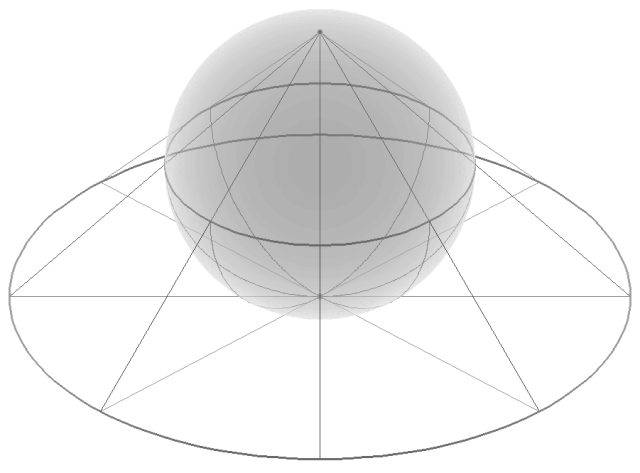
\includegraphics[scale=0.2]{Stereographic_projection.png}
    \caption{Stereographic Projection}
    \label{fig:awesome_image}
\end{figure}

The below is the standard picture for stereographic projection. We may replace the north pole and south pole with any pair of antipodal points, thereby associating any $ y \in \IS^n - \{ -x \}$ with a point on $T_x \IS^n$ for each $x$. This determines the map $f : \IS^n \times \IS^n - A \to E(\tau)$. $f$ identifies the zero section $\IS^n \subset E(\tau)$ with the diagonal $\Delta$ since the stereographic projection from $-x$ projects $x$ to itself. The homeomorphism gives us the first isomorphism 
$$ H^*(E, E_0) \iso H^*(\IS^n \times \IS^n, \IS^n \times \IS^n - \Delta) $$
Now note that $\IS^n \times \IS^n - \Delta$ deformation retracts to $A$. Here we present the picture for $n = 1$: 
In general, a little thought shows that $\IS^n \times \IS^n - \Delta$ can be seen as a trivial fiber bundle $A \times \IR^n$ over $A$. We can simply homotope each fiber to a point since $\IR^n$ is contractible. The homotopy gives us the second isomorphism
$$ H^*(\IS^n \times \IS^n, \IS^n \times \IS^n - \Delta) \iso H^*(\IS^n \times \IS^n, A) $$

Finally to show that the Euler class $e(\tau) = \phi^{-1}( u \cup u)$ is twice a generator $\alpha \in H^n(\IS^n; \IZ)$, it suffices to show that the Thom class $u \cup u$ is twice a generator of $H^{2n}(E, E_0)$ since $\phi : H^n(\IS^n; \IZ) \to H^{2n}(E, E_0)$ is an isomorphism, which in particular sends generators to generators. Under the homeomorphism $f$ we can view $\pi$ as the projection $\IS^n \times \IS^n \to \Delta$ given by $(x, y) \mapsto (x, x)$. Note that $H^{n-1}(\IS^n \times \IS^n, \Delta) \iso H^{n-1}(E, E_0) = 0$. The long exact sequence of the pair $(\IS^n \times \IS^n, \Delta)$ gives 
$$ 0 \to H^n(\IS^n \times \IS^n, \Delta) \to H^n(\IS^n \times \IS^n) \to H^n(\Delta) \to 0$$
Let $p_1, p_2 : \IS^n \times \IS^n \to \IS$ be projection to the first and second components respectively. Kunneth's theorem tells us that 
$H^n(\IS^n \times \IS^n)$ is generated by $p_1^*(\alpha), p_2^*(\alpha)$. If $\iota : \Delta \to \IS^n \times \IS^n$ denotes the inclusion map, then $$\iota^*(p_1^*(\alpha)- p_2^*(\alpha)) = \iota^*(p_1^*(\alpha)) - \iota^*(p_2^*(\alpha)) = (p_1 \iota)^* \alpha - (p_2 \iota)^* \alpha = 0$$
since $p_1 \iota = p_2 \iota$. Therefore by exactness of the sequence, $p_1^*(\alpha) - p_2^*(\alpha) \in H^n(\IS^n \times \IS^n, \Delta)$, identified as a subgroup of $H^n(\IS^n \times \IS^n)$. $H^n(\IS^n \times \IS^n, \Delta) \iso \IZ$, so $p_1^*(\alpha) - p_2^*(\alpha)$ must be a generator, since $(1, -1)$ is not a multiple of any $(a, b)$ with $a > 0, b> 0$. Therefore, $p_1^*(\alpha) - p_2^*(\alpha)$ corresponds to the Thom class $u|_E$ of $\tau$ up to sign. Now $u \cup u = (p_1^*(\alpha) - p_2^*(\alpha))^2 = - p_1^*(\alpha) \cup  p_2^*(\alpha) - p_2^*(\alpha) \cup  p_1^*(\alpha)$. When $n$ is even, we have that $p_1^*(\alpha) \cup  p_2^*(\alpha)$ commutes with $p_2^*(\alpha) \cup  p_1^*(\alpha)$, and hence $u \cup u$ is twice a generator of $H^n(\IS^n; \IZ)$. As a corollary, $\tau$ possesses no non-trivial sub-bundles since if so, then the Euler class should vanish. 


\begin{thebibliography}{9}


\bibitem{Milnor}
  J. Milnor, J. Stasheff, \textit{Characteristic classes}, Annals of mathematics studies, Princeton university press, Number 76, 1978
\end{thebibliography}



\end{document}
